\tikzset{every picture/.style={line width=0.75pt}} %set default line width to 0.75pt        
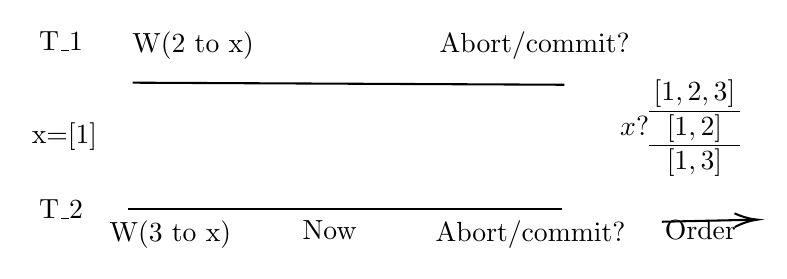
\begin{tikzpicture}[x=0.75pt,y=0.75pt,yscale=-1,xscale=1]
%uncomment if require: \path (0,300); %set diagram left start at 0, and has height of 300

%Straight Lines [id:da9500410641573396] 
\draw    (62.56,29) -- (270.56,30) ;
%Straight Lines [id:da7796185686481738] 
\draw    (60.56,90) -- (269.56,90) ;
%Straight Lines [id:da7329480179958066] 
\draw    (317.56,96) -- (361.56,95.04) ;
\draw [shift={(363.56,95)}, rotate = 178.75] [color={rgb, 255:red, 0; green, 0; blue, 0 }  ][line width=0.75]    (10.93,-3.29) .. controls (6.95,-1.4) and (3.31,-0.3) .. (0,0) .. controls (3.31,0.3) and (6.95,1.4) .. (10.93,3.29)   ;

% Text Node
\draw (16,3) node [anchor=north west][inner sep=0.75pt]   [align=left] {T\_1};
% Text Node
\draw (16,84) node [anchor=north west][inner sep=0.75pt]   [align=left] {T\_2};
% Text Node
\draw (61,3) node [anchor=north west][inner sep=0.75pt]   [align=left] {W(2 to x)};
% Text Node
\draw (50,94) node [anchor=north west][inner sep=0.75pt]   [align=left] {W(3 to x)};
% Text Node
\draw (209,3) node [anchor=north west][inner sep=0.75pt]   [align=left] {Abort/commit?};
% Text Node
\draw (207,94) node [anchor=north west][inner sep=0.75pt]   [align=left] {Abort/commit?};
% Text Node
\draw (317.56,94) node [anchor=north west][inner sep=0.75pt]   [align=left] {Order};
% Text Node
\draw (143,94) node [anchor=north west][inner sep=0.75pt]   [align=left] {Now};
% Text Node
\draw (12.5,47) node [anchor=north west][inner sep=0.75pt]   [align=left] {x=[1]};
% Text Node
\draw (296,25) node [anchor=north west][inner sep=0.75pt]   [align=left] {$x? \begin{array}{@{\,}c@{\,}}    [1,2,3]\\    \hline    [1,2]\\    \hline    [1,3]  \end{array} $};
\end{tikzpicture}